\documentclass{beamer}
\usepackage{textcomp}

\usepackage{graphicx}
\graphicspath{{./images/}}

\title[crisis]{Why there are no secure messaging apps}
\subtitle{Or other obviously distributed problems}
\author[Author, Anders]{Dean F. Valentine Jr., Tox Developer}



\begin{document}
  \begin{frame}
      \frame{\titlepage}
  \end{frame}
  \section{What the fuck happened?}
  \begin{frame}
      \frame{\sectionpage}
  \end{frame}
  \begin{frame}
      \frametitle{The internet has yet to develop a coherent system of sending messages between people.}
      So far, we have a few mature options:
      \begin{itemize}
          \item Proprietary, centralized services that host and coordinate (Skype, Discord, Etc.)
          \item End to End Encrypted, but still centralized messengers (Signal) (Matrix)
          \item Open source messengers that simply permit hosting your {\it own\/} centralized servers with logs of all chat (IRC)
      \end{itemize}
  \end{frame}
  \begin{frame}
      \frametitle{It makes you feel bad for the Chinese.}
      Basic, human messaging is the perfect application for distributed systems. It is a process
      that, in principle, should require only the parties that intend to do it. Beyond NAT traversal, the
      idea that any other servers need to be involved in transporting your text messages to another human
      being is incomprehensible.
  \end{frame}
  \begin{frame}
      \frametitle{All of these messaging systems have one or more of the following flaws:}
      \begin{itemize}
          \item They allow the hoster of the service to collect chatlogs.
          \item They allow the designated relay to collect all metadata.
          \item They enhance the censhorship capabilities of powerful actors by committing everyone to a single server/service.
          \item They require trusting the service hoster, in general, not to be a dick.
      \end{itemize}
  \end{frame}
  \begin{frame}
      \frametitle{So, why has the internet --- a technology for instant communication --- not created a good platform for actual communication?}
  \end{frame}
  \begin{frame}
      \frametitle{The answer is: There is no incentive to do it.}
      Any disributed platform that truly solved this problem would have no avenue for the creator to benefit from their 
      position as developer.
  \end{frame}
  \begin{frame}
      \frametitle{Consider what there would be left if someone actually did a good job in protecting groupchat communication:}
      \begin{itemize}
          \item There would be no way for the NSA or CCAC to spy on their citizens :(
          \item There would be no way for a company to sell chatlogs to third parties :(
          \item Metadata collection and parsing the userbase for relationships would be difficult :(
          \item There would be no way for infrastructure owners to silence people they didn't like :(
      \end{itemize}
      Clearly it would be very unfortunate if anyone ever {\it did\/} come up with a good messanger app.
  \end{frame}
  \begin{frame}
      \frametitle{After all, consider all the GOOD that has come out of services like Discord :D}
      \begin{itemize}
          \item Your government now has a collection of all of its citizens correspondences so they can Stopping Terrorism{\texttrademark}
          \item It is infinitely easier for private actors to learn what, and when, and with whom you communicate
          \item Sending a secure E2E Encrypted message to even a single individual requires trusting a third party with the metadata and using proprietary software
          \item And for most good groupchatting, these services now provide a nice compulsion for backdoored proprietary software to be included even on your linux machines :D
      \end{itemize}
  \end{frame}
  \section{I think we can all agree this development has been great. But what should we look out for to make sure this powerbalance is never upset?}
  \begin{frame}
      \frame{\sectionpage}
  \end{frame}
  \begin{frame}
      \frametitle{Well, let's consider what a BAD messaging app would look like.}
      \begin{itemize}
          \item An EVIL messaging app might avoid servers as much as possible, relying on trustless meshnets and self organizing swarms to connect users.
          \item It might use end to end encrypted messaging to make sure communications were authenticated and confidential.
          \item It might also prevent unassociated third parties from learning identifying information about users.
      \end{itemize}
  \end{frame}
  \begin{frame}
      \frametitle{Sadly, there seems to be a development on this front.}
      There is a messaging app called Tox that has been in development for the last few years with the sole
      purpose of depriving Paul Nakasone of his hard-earned civil liberties violations.
  \end{frame}
  \begin{frame}
      \frametitle{It is an open source, peer to peer messaging library that enables the exact kind of communications protocol that we've been worrying about.}
      Tox is an underbelly for several GUI/CLI clients like qTox, toxic, and Ricin that let people message each other over the
      WORST way possible. One that is end-to-end encrypted, completely peer to peer, and devoid of any centralized administrators.
  \end{frame}
  \begin{frame}
      Tox has solved the problem of fully, non-federated peer to peer messaging by using a Distributed Hash Table to manage userid's and public keys.
      \begin{enumerate}
        \item First, clients generate a long-term public key used as a ``Tox Address''.
        \item These IDs are announced to the network via onion routing.
        \item In order to talk to a Tox user, one sends a friend request to that Tox Address over the onion network.
        \item Once they accepts the friend request over that onion network, both hosts negotiate a second Public/Private keypair for direct IP---IP communication.
        \item They announce those private temporary public keys to the self-organizing swarm of tox nodes, and use them to find each other and communicate.
        \item If the users cannot directly connect to one another's PC's, they use NAT Traversal over those messenger nodes in the network to bypass this.
      \end{enumerate}
  \end{frame}
  \begin{frame}
      \frametitle{Fortunately, the current network has several problems.}
      \begin{itemize}
          \item There is no offline messaging; meaning, you can't send messages to a friend while they're offline, turn your computer off, and still have them arrive.
          \item The groupchats are not persistent --- Just like IRC, you can't send messages if you don't have a bouncer that retrieves them automatically.
      \end{itemize}
  \end{frame}
  \begin{frame}
      \frametitle{Unfortunately, these things will not be a problem forever.}
      Freenet has already solved the problem of offline, anonymous, decentralized data storage and a Rust or C implemmentation would make the above features trivial.
  \end{frame}
  \section{What should I NOT do to help prevent this from happening?}
  \begin{frame}
      \frame{\sectionpage}
  \end{frame}
  \begin{frame}
      \frametitle{I think it'd be a good idea to explain exactly what we shouldn't be doing to prevent this freedom situation from getting worse.}
  \end{frame}
  \begin{frame}
      \frametitle{There are public repositories on github for both the rust and C toxcore implemmentations.}
      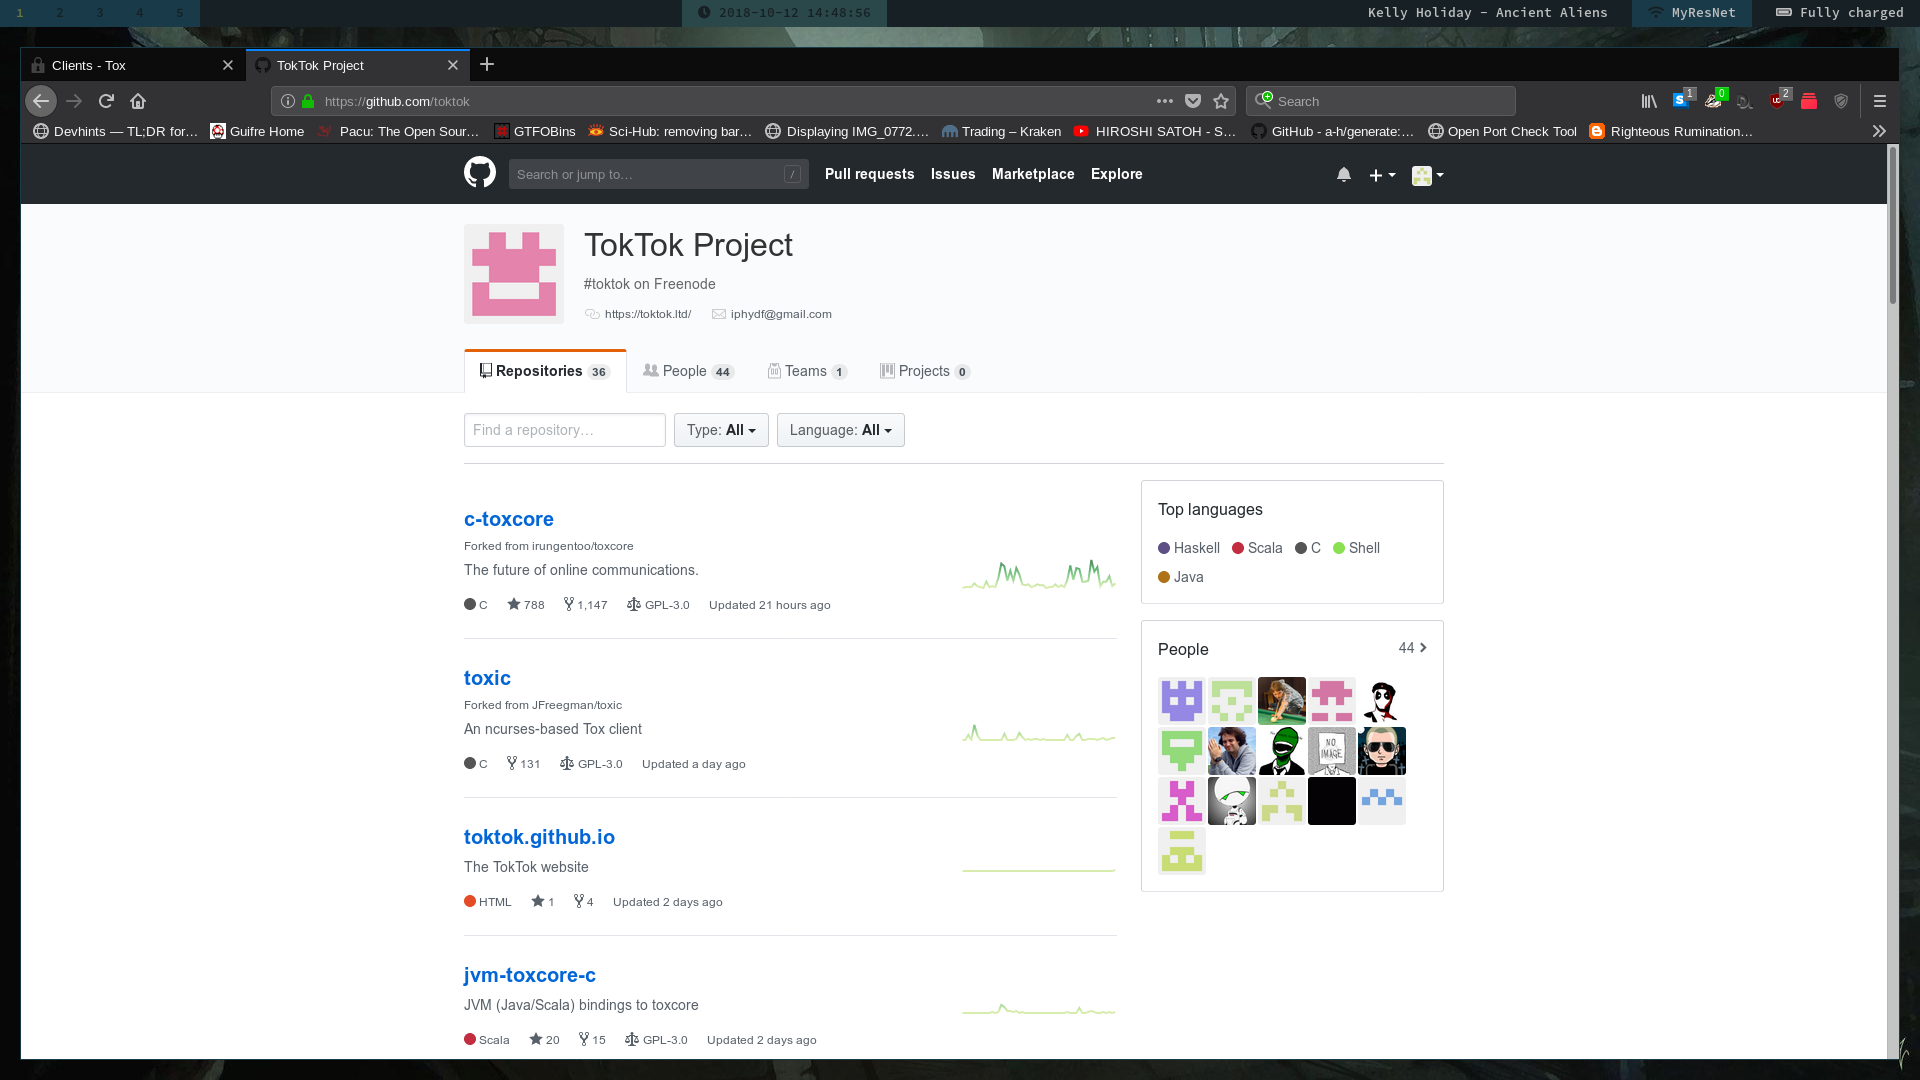
\includegraphics[width=\textwidth]{tox-github}

      {\bf DO NOT CONTRIBUTE TO THESE.}
  \end{frame}
  \begin{frame}
      \frametitle{Here is list of some of the things you SHOULDN'T contribute to that above github organization, TokTok, at \url{https://github.com/toktok/}:}
      \begin{itemize}
          \item The marked work on new features, like New Groupchats, and Offline messaging
          \item Clear, concise, specific bug reports or suggestions in the issue box
          \item Easy fixes for any of the issues in the c-toxcore or rs-toxcore issue list.
          \item Useful, efficient, self-documenting code improvements
          \item Improved or new unit and integration tests
      \end{itemize}
      And {\it DEFINITELY\/} don't help improve any of the several interfaces and clients like Toxic, qTox, Toxygen, Antox, and Antidote, by improving their ease of
      use or encouraging design improvements.
  \end{frame}
  \begin{frame}
      If you're not comfortable programming or using git, you can still mess up by:
      \begin{itemize}
          \item Contributing to the wiki at \url{https://wiki.tox.chat/}
          \item Using github's edit feature to submit pull requests for the website at \url{https://tox.chat}
          \item Improving or clarifying documentation of Tox's core protocol specification
          \item Shilling it to other programmers or users to the project, as I am doing now
      \end{itemize}
  \end{frame}
  \begin{frame}
      Remember --- Only hard libertarians, tech people and stallmanites would go through the agony and social discomfort of installing or recommending a second chat service.
      Think of all the cool funny messages Discord shows you when you're loading its spyware. 
      Think of all the targeted advertising. What would you do without targeted advertising?
  \end{frame}
% etc
\end{document}
